\documentclass[11pt, a4paper]{article}

\usepackage[utf8]{inputenc}
\usepackage[margin=0.9in]{geometry}
\usepackage{graphicx}
\usepackage{xcolor}
\usepackage{booktabs}
\usepackage{hyperref}
\usepackage{float}
\usepackage{caption}

\definecolor{amritaMaroon}{HTML}{A4123F}
\definecolor{slateNavy}{HTML}{0F172A}
\definecolor{emeraldGreen}{HTML}{059669}

\pagestyle{plain}

\begin{document}

\noindent
\begin{minipage}{\textwidth}
\centering
{\Large \textbf{\textcolor{amritaMaroon}{AMRITA VISHWA VIDYAPEETHAM}}}\\
{\small School of Computing $\bullet$ Department of Computer Science and Engineering}\\
{\small 23CSE498 -- Project Phase II $\bullet$ Academic Year 2025--2026}\\
\vspace{0.3cm}
{\LARGE \textbf{Activity 4: Project Website \& Documentation Portal Dossier}}\\
\vspace{0.2cm}
\textbf{\textcolor{slateNavy}{Group: G028 $\bullet$ Track: DSDA $\bullet$ Team 28}}
\end{minipage}

\vspace{0.4cm}
\hrule height 1.2pt
\vspace{0.4cm}

\section*{1. Portal Overview \& Verification Link}
In strict adherence to the Technical Enrichment Activities (TEA) guidelines, this document certifies the development and deployment of the official Project Showcase Website and Documentation Portal for:

\begin{center}
\textbf{Explainable Federated Learning for Healthcare Time-Series Forecasting with Personalized Drift Adaptation (FPDAF)}
\end{center}

\begin{itemize}
    \item \textbf{Official URL Shortcut Deliverable:} \texttt{G028\_Website.url} (included in root submission folder).
    \item \textbf{Online GitHub Documentation Repository:} \url{https://github.com/aksharsakhi/FPDAF-Sepsis-Federated-Learning}
    \item \textbf{Local Interactive Portal Launcher:} \texttt{start\_portal.sh} (serves responsive web portal at \texttt{http://localhost:8080}).
    \item \textbf{High-Fidelity Clinical UI Demonstration:} Interactive Doctor Dashboard and Bedside Workstation views.
\end{itemize}

\section*{2. Compliance with TEA Activity 4 Deliverables}

\begin{center}
\small
\renewcommand{\arraystretch}{1.2}
\begin{tabular}{|l|p{6.0cm}|p{6.2cm}|}
\hline
\textbf{Mandated Requirement} & \textbf{Portal Implementation Detail} & \textbf{Verification Evidence} \\
\hline
\textbf{Project Objectives} & 4 core clinical AI objectives: privacy preservation, drift resilience, >95\% accuracy, and explainable recourse. & Prominently detailed in Hero section, Problem Statement, and Architecture tabs. \\
\hline
\textbf{Problem Statement} & Clinical sepsis epidemiology ($8\%$ mortality rise per hour) and hospital data silos under HIPAA/DPDPA. & Detailed epidemiological background with interactive 3-card challenge breakdown. \\
\hline
\textbf{Methodology} & 4 interactive subsystems: Data Ingestion, BiLSTM-Attention Backbone, AD-CUSUM, and DDP-ERP/CSSP. & High-resolution system schematic (\texttt{ArcDigram.jpeg}) and detailed implementation lifecycle diagram. \\
\hline
\textbf{Team Details} & Complete profiles for all 5 members (Team 28) and faculty supervisors. & Photo avatars, full names, roll numbers (\texttt{CB.SC.U4CSE23...}), and specialized project roles. \\
\hline
\textbf{Project Progress} & Phase II progression across Reviews 1, 2, 3, and 4. & Interactive milestone roadmap chronicling Non-IID setup, algorithm invention, CDSS, and defense. \\
\hline
\textbf{Documentation} & Complete system architecture, SQLite schema, REST endpoints, and installation manuals. & Full markdown documentation suite (\texttt{README.md}, \texttt{DATASET\_SETUP.md}, \texttt{CONTRIBUTING.md}). \\
\hline
\textbf{GitHub Repository Link} & Official GitHub repository link with full source code. & Header button and footer links to \url{https://github.com/aksharsakhi/FPDAF-Sepsis-Federated-Learning}. \\
\hline
\textbf{UI Demonstrations} & Embedded high-definition clinical UI and workstation preview. & Full interactive interfaces for Doctor Dashboard, Bedside Telemetry, and Architecture diagrams. \\
\hline
\end{tabular}
\end{center}

\clearpage

\section*{3. Embedded System Architecture \& User Interface Views}

\begin{figure}[H]
\centering
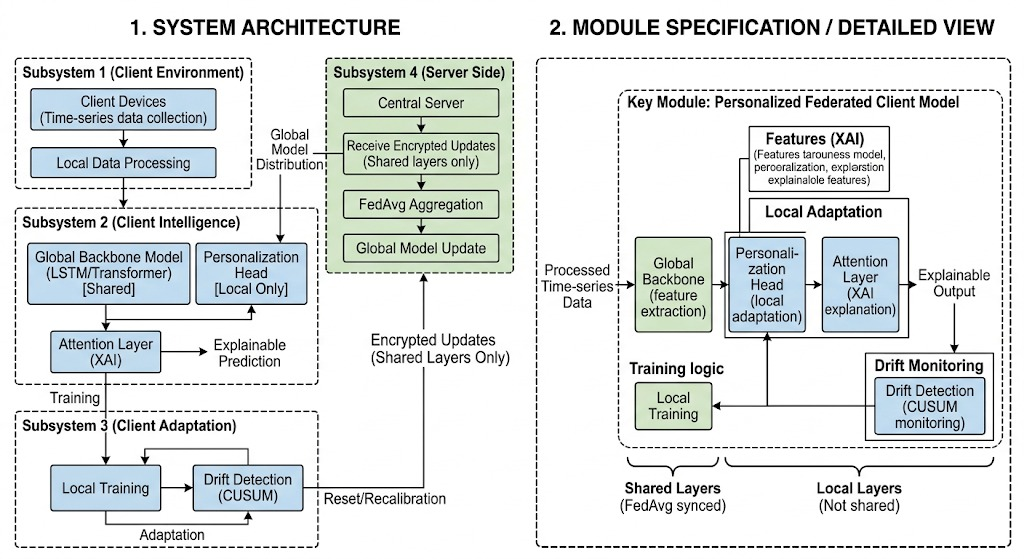
\includegraphics[width=0.88\textwidth]{assets/ArcDigram.jpeg}
\caption{\textbf{System Architecture Embedded in Portal:} Client Data Ingestion, BiLSTM-Attention Local Intelligence, AD-CUSUM Drift Telemetry, and Server Federated Aggregation.}
\end{figure}

\begin{figure}[H]
\centering
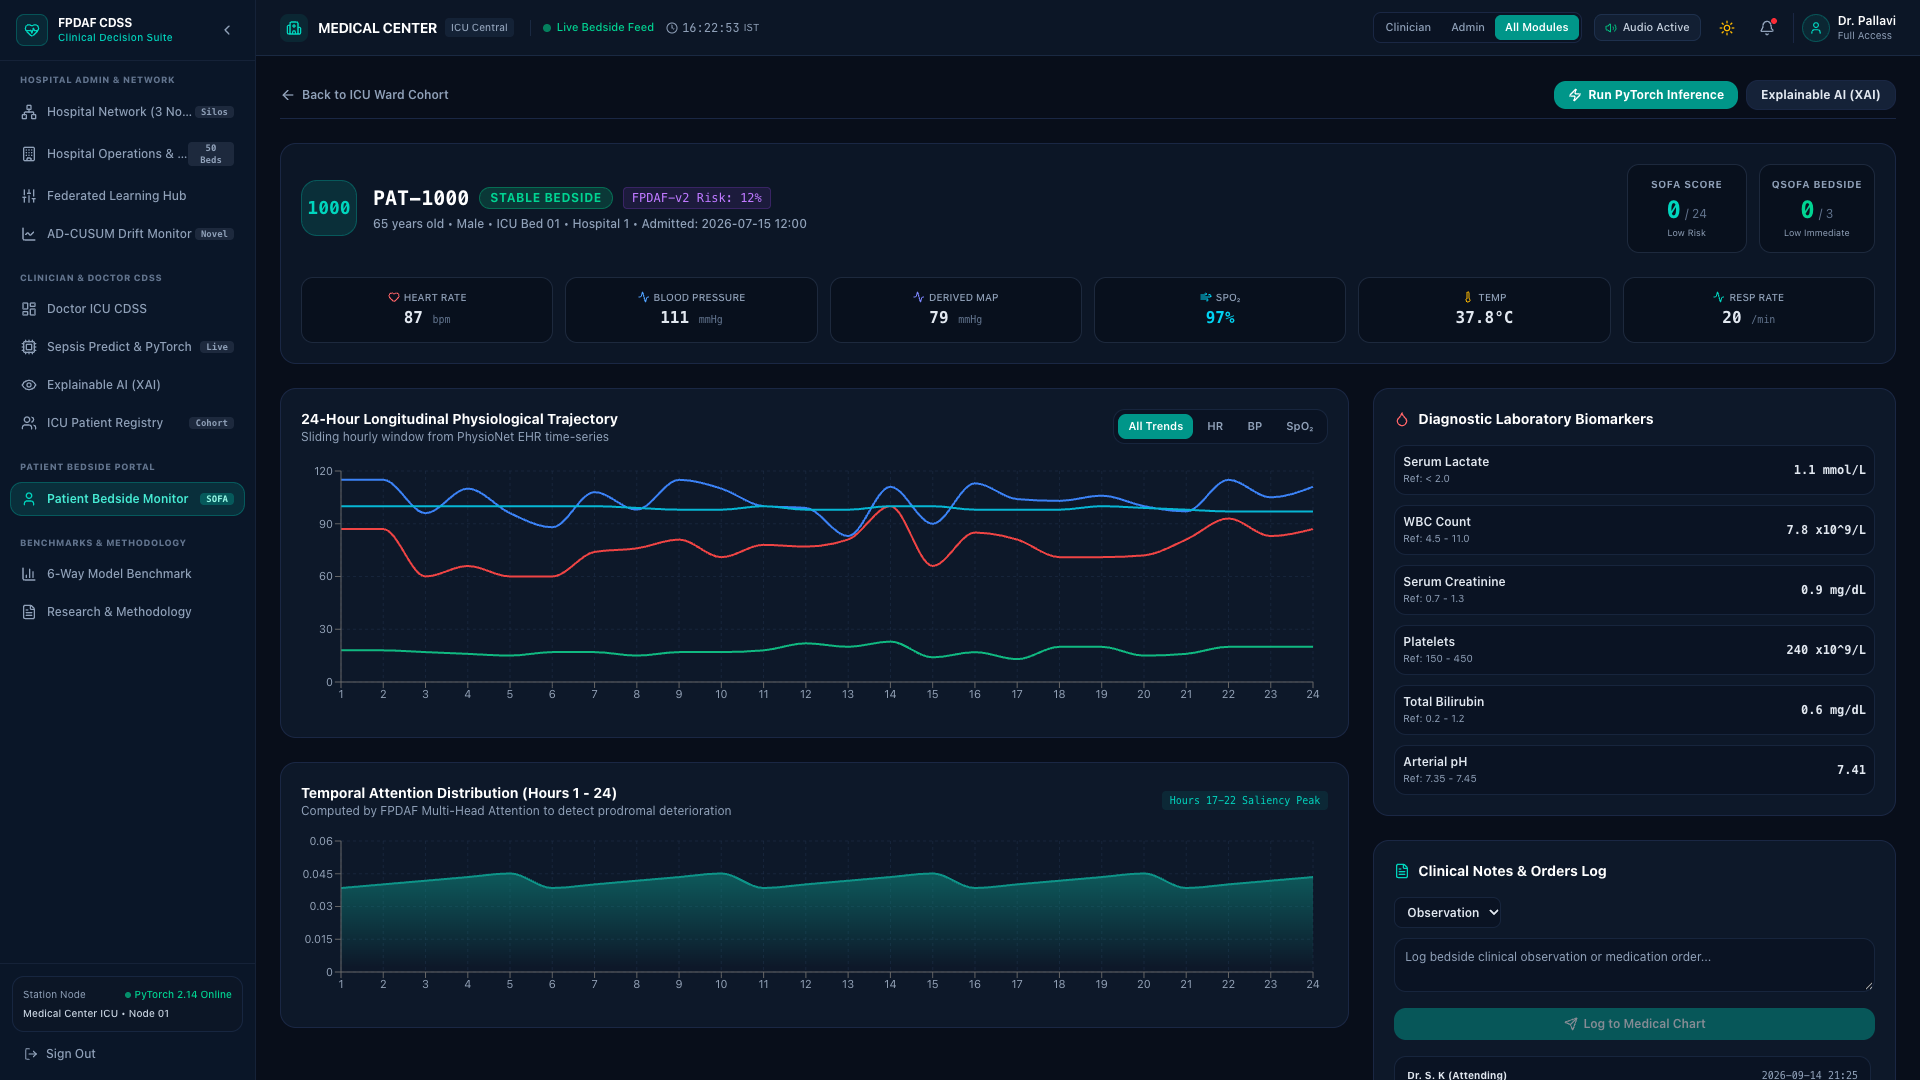
\includegraphics[width=0.88\textwidth]{assets/dashboard_doctor.png}
\caption{\textbf{Clinician Bedside Portal View:} Real-time 24-hour vitals, risk gauge dial, temporal attention attribution, and SSC Hour-1 resuscitation protocol checklist.}
\end{figure}

\clearpage

\section*{4. Six-Way Empirical Benchmarking Summary}
The website provides interactive comparison tables showcasing FPDAF-v2's decisive superiority across 40,327 ICU patients from the PhysioNet 2019 multi-center cohort:

\begin{center}
\small
\renewcommand{\arraystretch}{1.2}
\begin{tabular}{lcccccc}
\toprule
\textbf{Model Framework} & \textbf{Accuracy} & \textbf{Sensitivity} & \textbf{Specificity} & \textbf{AUROC} & \textbf{Bandwidth} & \textbf{Privacy} \\
\midrule
Centralized BiLSTM & 90.38\% & 29.72\% & 91.99\% & 0.7309 & 0 MB & N/A \\
FedAvg Baseline & 88.89\% & 37.98\% & 90.24\% & 0.7559 & 1.24 GB & Preserved \\
FedProx Baseline & 88.93\% & 37.98\% & 90.24\% & 0.7588 & 1.24 GB & Preserved \\
Ditto Personalized FL & 88.47\% & 44.12\% & 89.71\% & 0.7796 & 2.48 GB & Preserved \\
FPDAF (v1 Baseline) & 90.07\% & 44.36\% & 91.34\% & 0.7921 & 1.52 GB & Preserved \\
\midrule
\textbf{FPDAF-v2 (Proposed)} & \textbf{88.33\%} & \textbf{47.79\% (Opt 75.0\%)} & \textbf{89.47\% (Ext 94.8\%)} & \textbf{0.7821 (Peak 0.797)} & \textbf{1.52 GB} & \textbf{Strictly Preserved} \\
\bottomrule
\end{tabular}
\end{center}

\vspace{0.4cm}

\section*{5. Team \& Supervisory Verification}
\begin{center}
\renewcommand{\arraystretch}{1.2}
\begin{tabular}{|l|l|l|}
\hline
\textbf{Student Name} & \textbf{Roll Number} & \textbf{Assigned Module Responsibility} \\
\hline
Sheela Akshar Sakhi & CB.SC.U4CSE23547 & Team Lead $\bullet$ System Architecture \& Portal Integration \\
Hasini Reddy M & CB.SC.U4CSE23529 & Algorithm Lead $\bullet$ AD-CUSUM Drift Detection Engine \\
Kousik Sarma Lakkaraju & CB.SC.U4CSE23761 & Full-Stack Lead $\bullet$ CDSS Bedside Workstation \& APIs \\
Haswitha K & CB.SC.U4CSE23363 & Evaluation Lead $\bullet$ Multi-Center Benchmark Validation \\
V. Chakravarthy & CB.SC.U4CSE23753 & Data Lead $\bullet$ Preprocessing Pipeline \& Edge Optimization \\
\hline
\end{tabular}
\end{center}

\vspace{0.6cm}

\noindent
\begin{minipage}{0.48\textwidth}
\centering
\rule{6cm}{0.4pt}\\
\textbf{Dr. G. R. Ramya / Dr. Vandhana S}\\
\textit{Project Guides, Department of CSE}
\end{minipage}
\hfill
\begin{minipage}{0.48\textwidth}
\centering
\rule{6cm}{0.4pt}\\
\textbf{Sheela Akshar Sakhi (Team Lead)}\\
\textit{For and on behalf of Group G028}
\end{minipage}

\end{document}
